\documentclass[hyperref=unicode, presentation,10pt]{beamer}

\usepackage[absolute,overlay]{textpos}
\usepackage{array}
\usepackage{graphicx}
\usepackage{adjustbox}
\usepackage[version=4]{mhchem}
\usepackage{chemfig}
\usepackage[utf8]{inputenc}
\usepackage{caption}

\addtobeamertemplate{frametitle}{
	\let\insertframetitle\insertsectionhead}{}
\addtobeamertemplate{frametitle}{
	\let\insertframesubtitle\insertsubsectionhead}{}

\makeatletter
\CheckCommand*\beamer@checkframetitle{\@ifnextchar\bgroup\beamer@inlineframetitle{}}
\renewcommand*\beamer@checkframetitle{\global\let\beamer@frametitle\relax\@ifnextchar\bgroup\beamer@inlineframetitle{}}
\makeatother
\setbeamercolor{section in toc}{fg=red}
\setbeamertemplate{section in toc shaded}[default][100]

\usepackage{fontspec}
\usepackage{unicode-math}

\usepackage{polyglossia}
\setdefaultlanguage{czech}

\def\uv#1{„#1“}

\mode<presentation>{\usetheme{default}}
\usecolortheme{crane}

\setbeamertemplate{footline}[frame number]

\makeatletter
\setbeamertemplate{navigation symbols}{}


\title{Chemické pokusy - videa pro Commons}

\subtitle{Wikikonference 2024}
\author{Zdeněk Moravec \\ zdenek.moravec@wikimedia.cz}

\titlegraphic{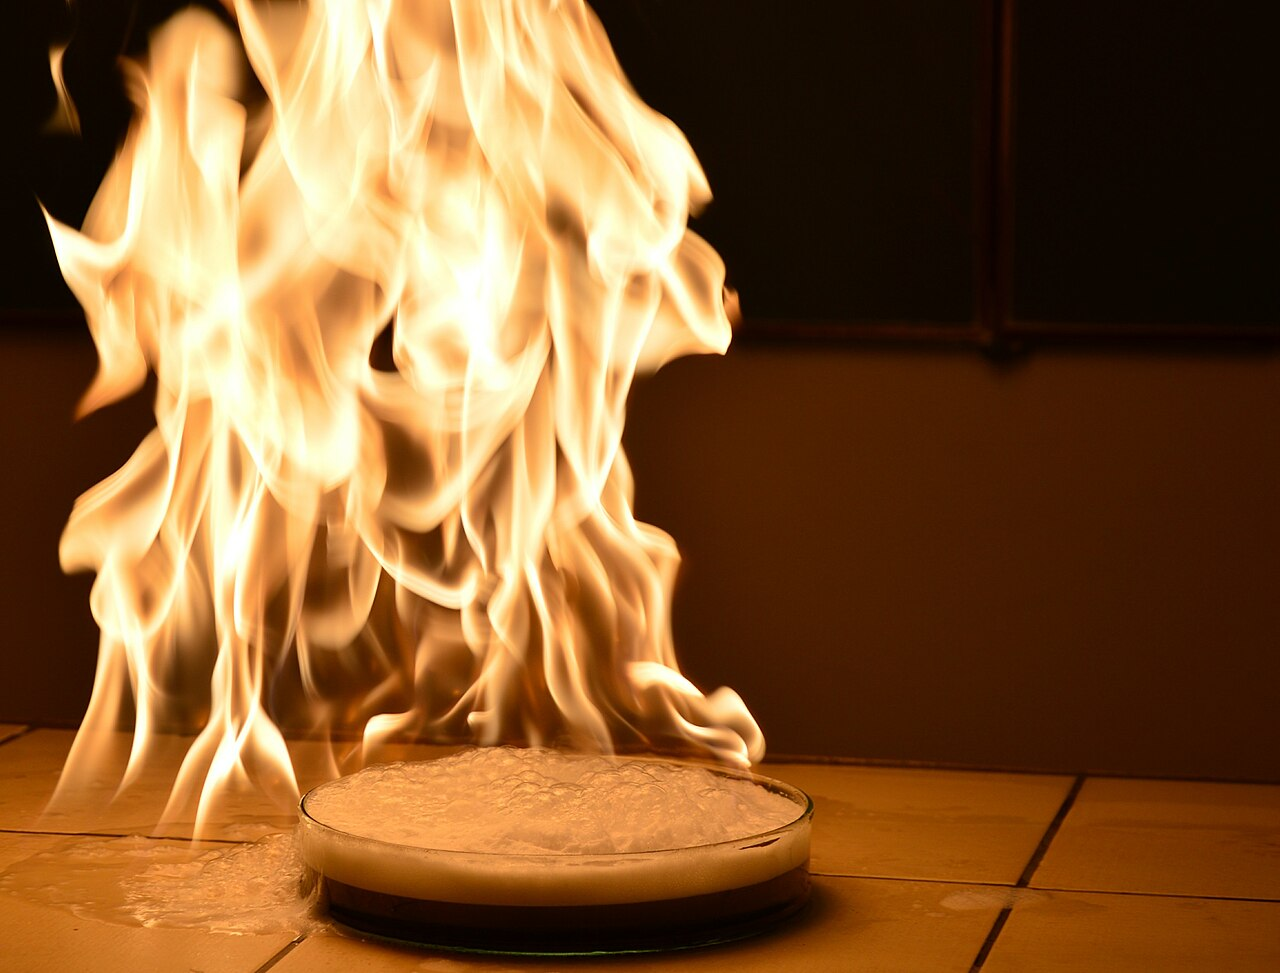
\includegraphics[height=.35\textheight]{img/intro.jpg}}

\date{}

\begin{document}

\begin{frame}
	\titlepage
\end{frame}

\section{Wikimedia Commons}
\frame{
	\frametitle{}
	\vfill
	\begin{columns}
	\begin{column}{.75\textwidth}
	\begin{itemize}
		\item Celkem více než 110 miliónů souborů (569 TB).\footnote[frame]{\href{https://commons.wikimedia.org/wiki/Special:MediaStatistics}{Wikimedia Commons -- Media statistics}}
		\item Obrázků je více než 101 miliónů (390 TB).
		\item Videí je pouze necelých 332 000 (30 TB).
	\end{itemize}
	\end{column}
	
	\begin{column}{.3\textwidth}
		\begin{figure}
			\adjincludegraphics[width=\textwidth]{img/Commons-logo.png}
		\end{figure}
	\end{column}
	\end{columns}
	\vfill
}

\section{Chemické pokusy}
\frame{
	\frametitle{}
	\vfill
	\begin{itemize}
		\item Pokusy jsou důležitým doplňkem výuky chemie, fyziky a dalších předmětů.
		\item Realizace složitějších experimentů je v prostředí základních a středních škol obtížná.
		\item Jako částečná náhrada mohou sloužit fotografie a videa.
		\item Výhodou zveřejnění videí na Commons, např. oproti Youtube, je jejich dostupnost pod licencí Creative Commons.
	\end{itemize}
	\vfill
}

\end{document}
